
Using the similarity matrix generated, a graph of document similarities is generated: Each document is represented as a node, which is connected to other documents in the graph by edges representing the similarity measure of the two documents.

\subsubsection {Querying Functionalities}
\label{sec:querying_functionalities}
The nodes of the graph are generated from the results of a database query supplied by the user, who can search either by keyword, by named entity (entered in double quotes, e.g.\ \code{"Castro"}) or by a combination of both in the same query. Likewise, the user may select a range of years to search in (e.g.\ retrieve documents only occurring between 1970 and 1975), as well as select only certain types of documents to be searched (e.g.\ retrieve only documents of type \code{SPEECH} or \code{INTERVIEW}). The documents most relevant to the current query are displayed, the number of the documents displayed being specified by the user (e.g.\ display the 25 most relevant documents), and edges connecting each document are drawn based on the similarity measures relating each document to each other.

\subsubsection {Presenting Results}
\label{sec:presenting_results}
After submitting a query, the graph is drawn, in which the relevance measure of each document to the current query is represented by the absolute size of the node representing the document in question: The larger the node, the more relevant it is to the current query. The type of document represented by the node is represented by its shape: \note{Add symbol key!}

By default, the edges drawn are determined by the absolute similarity measure: If the similarity measure of two documents is greater than a user-adjustable edge threshold, an edge is drawn between them. The higher the absolute similarity of the two documents, the thicker the edge. However, the user may set the method of edge generation to display edges according to the relative similarity of the documents shown: According to the user-specifiable edge density, the more similar two documents are compared to the similarities of other documents, the thicker the edge.

By adjusting the edge threshold (for absolute similarity) or the edge density (for relative similarity) the user can adjust the level of detail represented by the graph. This allows the user to both discern relationships between documents which are not very similar to each other, and to prune out relatively weaker relationships between documents which are very similar to each other.

\pagebreak
%\begin{figure}[t]
%\centering
%\caption{GUI}
%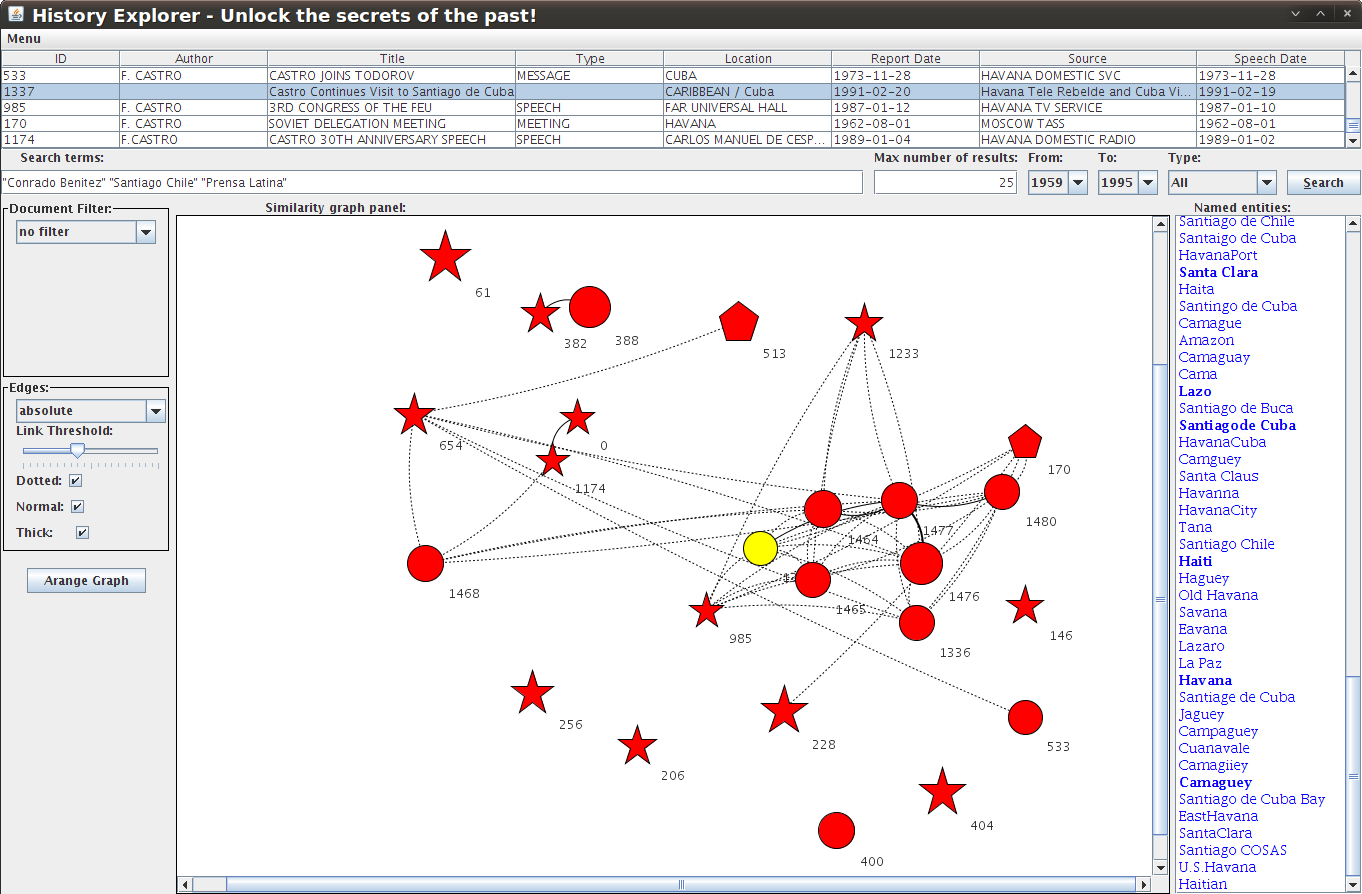
\includegraphics[width=160mm]{gui.png}
%\end{figure}

\subsubsection {Navigating Through Results}
\label{sec:navigation_through_results}
The graph, query input and display options are integrated into an interactive graphical front-end: Clicking on the node in the graph with the mouse selects it and displays in a sidebar the named entities associated with the document the node represents. Boldface entries represent named entities in the given document, while the non-boldface entries represent named entities similar to the boldface named entities in the document according to the string kernel similarity measure. For example, the named entity \textbf{\lingform{Castro}} may also return the similar named entities \lingform{Fidel}, \lingform{Fidel Castro} and \lingform{Dr. Fidel}. Additionally, by right-clicking on the node, the user may choose to view the document metadata (e.g.\ document type, date or location) or the document text itself. In the text, the named entities recognized in the text are displayed in a color associated with the type of entity, e.g.\ red for persons, green for organizations and blue for locations.

Additionally, a vertex filter may be applied, enabling the user to display only nodes of a specified distance from a selected node, e.g.\ displaying only the nodes directly connected to the current node (a distance of 1) or displaying nodes which are connected to the selected node through at most one node (a distance of 2). This may be done in real-time, i.e.\ after applying a distance filter, the user may select a node in the graph to view an updated graph of all nodes satisfying the distance criterion for the newly-selected node. This feature allows the user to draw ``sub-graphs'' of the main graph in real time, allowing the user to focus on a particular cluster of documents and thus allowing the user even greater control over the search results.